\section{Helpfulness Prediction}
Our ambitious goal was that of building a model able to predict the helpfulness of a review, looking only at the text of the review itself.
To create such a model, we needed firstly to convert the text in a machine-readable format, performing a process called \textit{feature extraction}.
Then we tried different models, in order to find the one that best fits our needs eventually selecting the best one.

\subsection{Feature Extraction}
Seen the complexity of the problem we decided to use a \textit{Word Embedding} technique, called \textit{Word2Vec}, that is able to convert a word in a vector of real numbers
while preserving the semantic meaning of the word itself. We used the \textit{Gensim} library to perform this task using the following parameters:
\begin{itemize}[noitemsep, leftmargin=*]
    \item \textbf{Size}: 30
    \item \textbf{Window}: 5
    \item \textbf{Min Count}: 2
    \item \textbf{Workers}: -1
\end{itemize}
As a consequence, each word is represented by a vector of 30 real numbers. The average of the vectors of all the words in a review is the vector representation of the review.

\subsection{Models}
We tried three different models: \textit{Random Forest}, \textit{Support Vector Regressor (RBF kernel)} and \textit{MLP}.
We used the \textit{Scikit-Learn} library to perform the training and the testing of the models. Specifically for this last step
we used the \textit{GridSearchCV} class, that performs a cross-validation on the training set, in order to find the best parameters for the model.
The results are show in Table \ref{tab:model_results} and supported by Figure \ref{fig:model_results}.

\begin{table}[H]
    \footnotesize
    \centering
    \caption{Model Results}
    \label{tab:model_results}
    \begin{tabular}{|c|c|c|c|}
        \hline
        Model & MSE & RMSE & R\textsuperscript{2} \\
        \hline
        RF & 0.0259 & 0.1609 & 0.2532 \\
        SVR & 0.0279 & 0.1670 & 0.1955 \\
        MLP & 0.0282 & 0.1680 & 0.1858 \\
        \hline
    \end{tabular}
\end{table}

\begin{figure}[H]
    \centering
    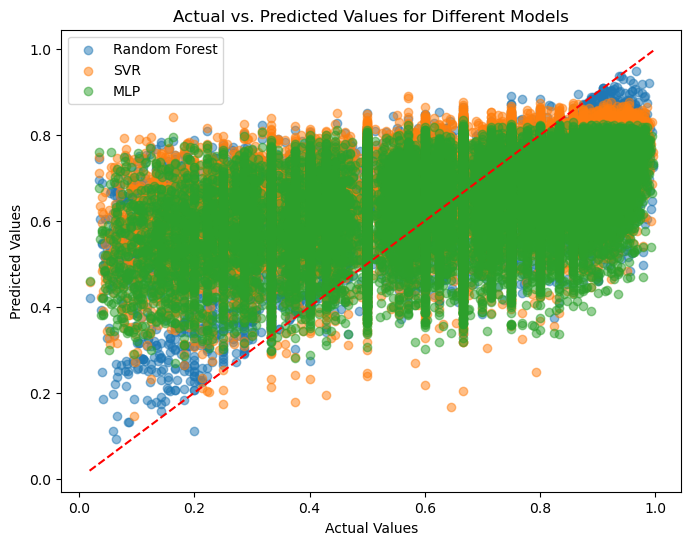
\includegraphics[width=0.48\textwidth]{./figures/model_results.png}
    \caption{Model Results}
    \label{fig:model_results}
\end{figure}

\noindent
As we can see from the graph and the metrics used, the Random Forest model outperforms the other models in terms of Mean Squared Error 
(MSE) and Root Mean Squared Error (RMSE). The Random Forest model achieved the lowest MSE of approximately 0.026 and RMSE of approximately 
0.161, indicating that its predictions are, on average, the closest to the actual values. 
This suggests that Random Forest has the best overall predictive performance among the three models.

\subsection{Results Interpretation}
Figure \ref{fig:model_best_scatter} and Figure \ref{fig:model_best_lines} help us in the results Interpretation.


\begin{figure}[H]
    \centering
    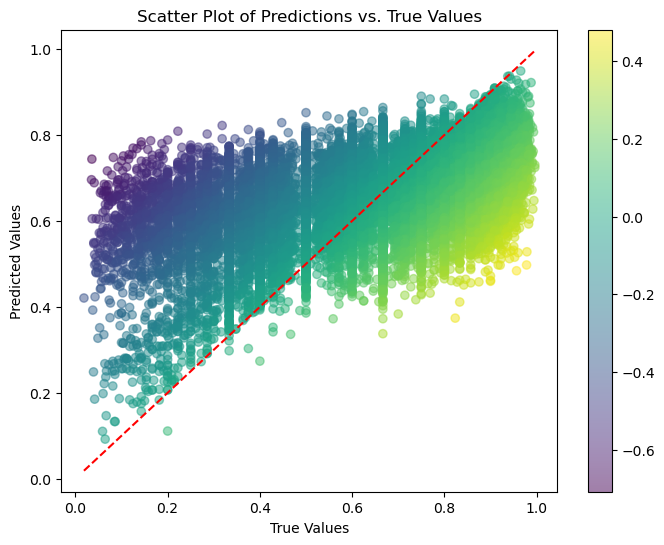
\includegraphics[width=0.48\textwidth]{./figures/model_best_scatter.png}
    \caption{Best Model Errors}
    \label{fig:model_best_scatter}
\end{figure}

\begin{figure}[H]
    \centering
    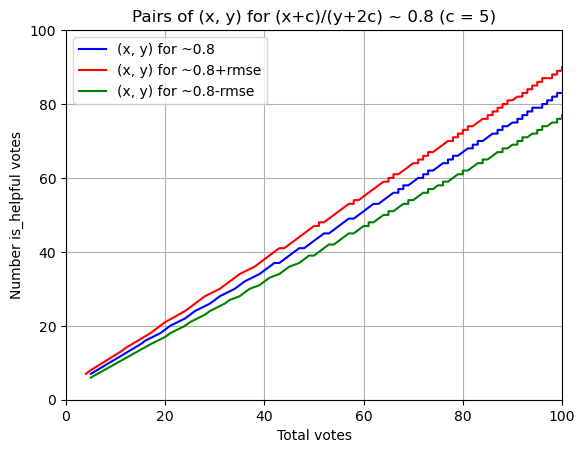
\includegraphics[width=0.48\textwidth]{./figures/model_best_lines.png}
    \caption{Best Model Errors Translation}
    \label{fig:model_best_lines}
\end{figure}




